\newpage

\chapter{Extended Market Analysis}
\label{ch-market}

In this chapter the performed extended market analysis is explained. The goal of the extended market analysis is to further investigate how an UAM system can best be implemented in Los Angeles. First, the general effects of congestion are described in \autoref{effects}, after which an analysis is done on how congestion in LA may be decreased (\autoref{decrease}). Then, the user needs are explained in further detail in \autoref{needs}. Section \ref{quantmarket} gives an explanation on how the available data of commuters is used and processed. Moreover, in \autoref{legislation} an estimation of legislation in 2050 is provided. Finally, in \autoref{comparisonmodesoftransport} a comparison in terms of energy usage is made between several existing modes of transport. 

\section{City Case Study}

Los Angeles (LA) is widely seen as the city with the worst congestion problem in the United States. Knowing the effects of the congestion will be of great importance in understanding how to solve this problem. Furthermore, understanding why commuters keep on using cars instead of existing public transport systems can provide an insight in how the UAM system should be designed, so that it answers the wishes and needs of possible users.

\subsection{Effects of Congestion}
\label{effects}
Congestion in major cities is not only inconvenient, but also brings along significant health problems. A standard vehicle drives most efficiently during cruise, but in case of congestion, the vehicle is mostly busy with either accelerating, decelerating or the engine is left idling. 

For example, a standard car emits gasses such as particulate matter (PM), nitrogen oxides (NO\textsubscript{x}) and carbon monoxide (CO). As particulate matter is extremely small, it can settle deep in someones lungs, which is extremely hazardous for someone's health. In addition to this nitrogen oxides, these have a negative influence on personal health as well. A usual symptom is tiredness and nausea. Moreover, it damages agricultural crops and other plants too. Carbon monoxide is a known cause of the increase of other greenhouse gases. Meaning it has a direct negative effect on the climate change \cite{cargasses}. 

The Environmental Protection Agency (EPA) has set the so called National Ambient Air Quality Standards (NAAQS) to provide public health protection. According to these standards the maximum concentration of PM2.5 annual mean, averaged over 3 years,
is 12 $\mu g / m^3$ \footnote{\url{https://www.epa.gov/criteria-air-pollutants/naaqs-table} [accessed 10.05.19]}. \autoref{fig:PMLA} shows the concentrations at peak traffic hours in LA in 2013. It can be seen that the concentrations of PM2.5 go far above 20 $\mu g / m^3$. It should be noted that these numbers are not averaged, however, it goes without question that these concentrations are extremely bad for the health of the community living close to these highways.  

\begin{figure}[h]
    \centering
    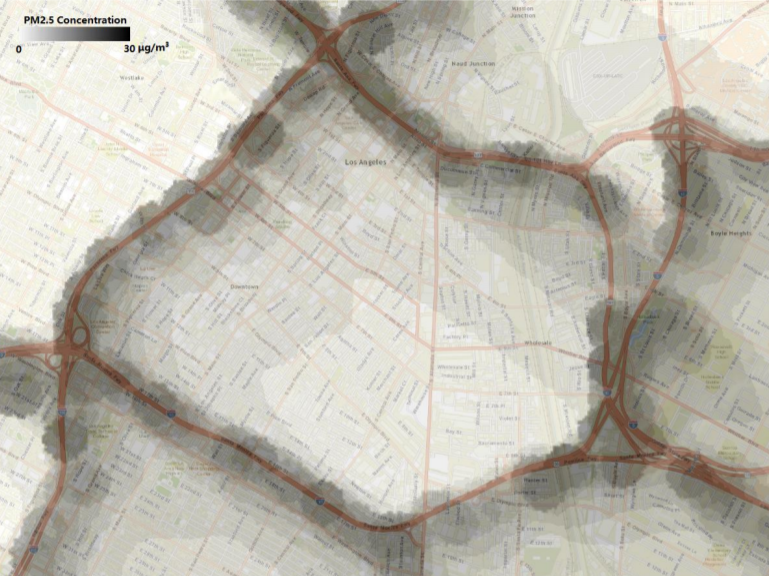
\includegraphics[width=0.75\linewidth]{Figures/PMLA.png}
    \captionsetup{justification=centering}
    \caption{Map of downtown LA showing PM 2.5 concentration in peak traffic in August 2013} \cite{pmlevelLA}
    \label{fig:PMLA}
    % this still needs to be edited
\end{figure}

\subsection{Ways to decrease congestion}
\label{decrease}
In LA, there have been multiple studies and proposals in order to try and decrease the congestion problem. The most recent study that is now taken into serious consideration, is a \$4 (USD) tax for cars travelling in a certain zone during peak hours. This so called 'Mobility Go Zone' \cite{mobilitygo} would be implemented in the most congested parts of LA to reduce the amount of people using cars and stimulating the use of public transport instead. In a feasibility study it was found that in 2035 this measure would decrease the amount of cars used during peak hours by 19\%, while increasing the use of other transit systems by 9\%. This decrease of car usage would decrease the vehicle hours travelled by almost 24\%. This gives an indication of the amount of passengers the UAM system should have to transport to significantly reduce the congestion and time that people spend in traffic jams. 

Furthermore, much research has been done into new public transport systems. In 2015, a study \cite{lightrail} investigated the effect on road congestion due to a proposed light rail connection in downtown LA. The results that were found suggested that the reduction in road congestion would be small and local, even though the overall transit use would increase. An important factor for the lack of improvement in the road traffic is that the percentage of people who would shift to the public transport system is relatively small compared to the total amount of car users. Also, possible new local congestion could occur at park-and-ride-facilities of the station. All in all, these effects are expected to take place on a local scale only. However, this should be taken into account during the development of the UAM system. Hubs or vertiports will probably attract extra traffic in their near surroundings. It should be avoided that this extra traffic causes congestion. In addition to this, to really make a serious impact on the total road congestion, the system should cover a large area. 

\subsection{User Needs}
\label{needs}
Based on an extended analysis, the primary transport related problem in Los Angeles is congestion. Congestion in Los Angeles is caused by the combination of 84\% of the daily commuters using a car and driving alone, and the fact that almost 46\% of the population of Los Angeles lives in urban areas surrounding Los Angeles. This shows that the frequent users will be the people who mainly use a form of private motorized transport to commute to work every day. This leads to the analysis of why the percentage of daily commuters using private transport is as high as it is. 

Problems with the LA Metro system also influence users to rely on private transport rather than public. One of the problems of the LA Metro system is the low amount of rail stations due to the very spread-out layout of Greater Los Angeles. The amount of rail stations in LA is a little over 110 \footnote{\url{https://media.metro.net/documents/8f0fe43e-da3b-4a10-bd8e-4cfd54e30eb3.pdf}[accessed 17.05.19]}, whereas the area of Greater Los angeles is 87,940 $km^{2}$ \footnote{\url{https://simple.wikipedia.org/wiki/Greater_Los_Angeles_Area}[accessed 17.05.19]} . This indicates that the reachability of the rail stations is bad, resulting in the need for a prior form of transport in order to get to the rail station. Even though the amount of bus stations in Greater Los Angeles is 20,000, the LA Metro system faces a reliability problem; 22.7\% of the buses in 2016 were late. This reliability problem paired with the low frequency of buses makes a 10 minute ride by car turn into a trip which can easily take 50 minutes by bus (due to waiting time, the lower average speed at which a bus generally drives compared to a car, and the amount of stops the bus makes along the way). Furthermore, the general image of the LA Metro system is bad due to the limited carrying capacity, which was clearly seen after the extension of the expo line (Santa Monica) and overcrowding of the trains, which resulted in the smell in the trains becoming bad and the trains becoming dirty; the general image of the LA Metro system became “cheap”. This consequently resulted in 30\% of the users feeling unsafe and staying away even after considering the fact that the LA Metro system is very safe compared to the neighbourhoods surrounding the various stations. Another reason why the LA Metro ridership is so relatively low compared to the expected ridership is due to the sense of control aspect experienced by the commuters. Acknowledging the fact that owning and driving a car provides users with a sense of “complete control”, as the user has the freedom to choose when and where to go without the need of checking any schedules (public transport) \footnote{\url{https://www.citymetric.com/transport/los-angeles-metro-great-so-why-aren-t-people-using-it-2742}[accessed 17.05.19]}. 

After the analysis of the main aspects which result in a low ridership rate of the LA Metro system, the main aspects which have to be considered by the design team are:
\begin{enumerate}
    \item Sense of Luxury : clean environment, aesthetics, level of technology, comfort
    \item Reliability and availability : waiting time, carrying capacity, amount of vehicles 
    \item Reachability 
    \begin{itemize}
        \item Hub-to-hub system : Commute distance to a hub  
        \item On demand system : Accuracy take-off and land locations
    \end{itemize}
    \item Sense of safety
    \item Commute time : Always lower than any other form of transport
    \item Sense of control
    \item Cost : ticket fare or cost per kilometer
    \item Integration within the city : with other modes of transport (public transport)
\end{enumerate}


\section{Quantitative Analysis of Market}
\label{quantmarket}
The worker population of Los Angeles metropolitan area can be considered the target group of this mobility system. They would be the likely users of the system. This metropolitan area consists of Los Angeles city and other areas.
Data from the "Census Transportation Planning Products" (CTPP) is used to identify travel patterns of the worker population. This data-set has information about the number of workers, their residence locations, their workplace location and the start time of the their commute \footnote{\url{https://ctpp.transportation.org/2012-2016-5-year-ctpp/} [accessed 08.05.19]}.\\\\
The residence locations of the workers are given in terms of "Public Use Microdata Areas" (PUMAs). A PUMA is geographical area that consists of about 100,000 to 200,000 residents. The use of a PUMA gives a relatively accurate indication of the starting point of a commute. It was found that a PUMA could not be used to classify workplace locations; the CTPP data did not have sufficient data concerning the workplace locations within a PUMA. Therefore, the workplace location of the workers are given in terms of "Principal Cities of the Metropolitan Statistical Area of Los Angeles". The Principal City is the most important city of the Metropolitan Area with a high percentage of working people in comparison to the residents. The locations of this principal cities was found on a map and this was translated to a location within a PUMA.\\\\
An inconvenience was that, in the data-set, Los Angeles city as a whole was considered as a principal city. It would have been better if it was sub-divided into regions within the city. It was found that Los Angles city had four main workplace areas; Downtown, Westwood, Koreatown and Hollywood. The number of working people in Los Angeles city was divided into these four areas. The ratio used to divide the people was found using another source \footnote{\url{http://ccdphila.maps.arcgis.com/apps/OnePane/basicviewer/index.html?appid=54a5a70269ba44b48efe1b9f3ffe35cb} [accessed 08.05.19]}. \\\\
The start time of the commute was between 5:00 am and 9:00 am in steps of one hour (e.g. 5:00, 6:00 ...). Because no accurate CTPP data for the evening rush hour is available, only the morning was observed and assumed this would also represent the evening. The original data-set was processed using Python, where a list of 10,000 routes was compiled for each time frame. Each route had information about the source, destination and the number of workers on that route for that time frame. A Google MAPS API (Application Programming Interface) was used to further find characteristics of the route. These characteristics include the distance, time taken in traffic and time taken without traffic. These metrics will enable the group to identify which routes are the most congested. \\\\
The visualisation of the PUMAs and the routes will help the team identify infrastructure patterns of the various systems. A MAP tool is made which outputs a map for each time-frame. The top $n$ (parameter) routes based on the gain metric are drawn on the map. The PUMAs are colour-coded based on their inflow flux. This is the number of people entering that specify PUMA in given time-frame. A darker red indicates a higher inflow flux. The locations of the major airports are also plotted on the map. 

\section{Legislation}
\label{legislation}
There is a huge market for Unmanned Aircraft Systems (UAS), often referred to as drones. They could for example be used for industrial inspection or aerial photography, but also to transport people. Officially, drones can only be used below navigable airspace. The question that often follows is: Who owns that airspace? The Federal Aviation Administration (FAA) has the exclusive authority to regulate all aircraft vehicles, manned or unmanned, within navigable airspace. The FAA defined navigable airspace as the airspace that is required for safe takeoff and landing of airplanes, combined with the airspace above the minimum flight altitudes. \footnote{\url{https://www.faa.gov/airports/engineering/airspace_analysis/} [accessed 08.05.19]}. So, new rules will have to be created to regulate the use of UAS in low-altitude airspace. Two years ago, a new program was started: The Unmanned Aircraft System (UAS) Integration Pilot Program (IPP). By bringing together the different governments with private parties, national and local interests are being identified. This is done by also taking into account security and privacy issues that might arise. The goal of the program is to increase the speed at which new rules are created and authorized\footnote{\url{https://www.faa.gov/uas/programs_partnerships/integration_pilot_program/} [accessed 08.05.19]}.

In addition to IPP, the FAA started in 2007 on modernizing the overall aviation system. This project is referred to as 'NextGen'. NextGen should lead to an aviation system which is safer, more efficient, has a higher capacity and predictability. The target of NextGen is to have all major components implemented by 2050\footnote{\url{https://www.faa.gov/nextgen/what_is_nextgen/} [accessed 08.05.19]}. The major changes will be in navigation and communication. By switching towards satellite-enabled navigation, optimum routes can be determined more easily, as it is much more accurate than ground-based navigation. Moreover, the new data communication system will allow for more quicker and easier communication in air traffic. In addition, it will reduce the risk of miscommunication that occurs due to radio messages over busy frequencies\footnote{\url{https://www.faa.gov/nextgen/how_nextgen_works/} [accessed 08.05.19]}.

It is clear from all the ongoing projects and their desired results that by 2050 major changes will have occurred in the overall legislation. In \autoref{fig:airmapla} it is shown which areas currently have to comply with specific FAA regulations. The type of regulation and size of the area depends on the airport under consideration. The map clearly shows that there is a need for new rules that apply to the low-altitude airspace underneath the navigable airspace. The system will adjust its flight routes such that it will comply with the new FAA regulations. Moreover, not only the location of airports influence the flight routes that the system will be using, also the location of hospitals with a helipad influence this. At any moment in time the system should not interfere with emergency helicopters. 

\begin{figure}[H]
    \centering
    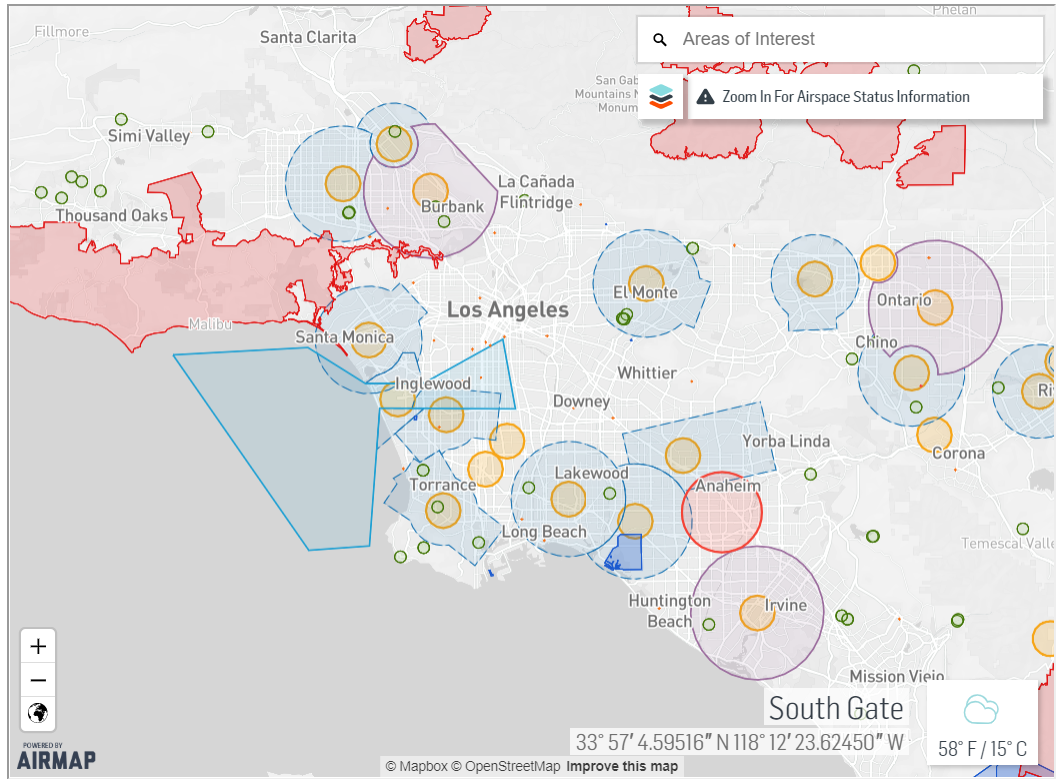
\includegraphics[width=0.75\linewidth]{Figures/AirMapLA.png}
    \captionsetup{justification=centering}
    \caption{Map of Los Angeles showing airports and corresponding zones in which certain FAA regulations have to be complied with \protect\footnotemark}
    \label{fig:airmapla}
\end{figure}

\footnotetext{\url{http://knowbeforeyoufly.org/air-space-map/} [accessed 09.05.19]}

Together, the new data communication system and satellite-based navigation, will make it possible to travel safely through low-altitude airspace. They do so, by providing very accurate data of current locations and estimated flight routes of all other vehicles that are in the air or will go into air. 




\section{Possible Other Solutions}
\label{comparisonmodesoftransport}
The trade off process, criteria and tools have been extensively discussed in the above sections. This was all done with the goal of selecting a suitable Urban Air Mobility system to tackle congestion and pollution issues in Los Angeles. One must also investigate other modes of transport which can help reduce congestion. The modes of transport can act as both competition or complement the system. The modes of transportation considered are cars, buses and trains. The Hyperloop concept is not considered as it aims to transport people over further distance than the Urban Air Mobility system \cite{hyperloopsucks}.
\subsection{Electric Cars}
Cars will also be a mode of transportation in 2050. These cars will likely be electric. This is done based on the the current development in the market of electric vehicles and the growing number of auto manufacturers introducing electric cars. The use of electric cars will decrease air pollution in Los Angeles and help the tackle climate change; provided the energy comes from a renewable source. \\
However, the team foresees that electric cars will not be able to solve the congestion problem in Los Angeles. A three-dimensional traffic system is needed help tackle traffic congestion in Los Angeles \footnote{\url{https://www.ericsson.com/en/blog/2018/6/we-need-three-dimensional-traffic-congestion-solutions} [accessed 17.05.19]}. Hypotheically, this is possible by having a three-dimensional network of roads; possible some tunnels in the city.   




With the projected population growth of LA, simply transitioning to a clean energy source will not provide a solution to this issue. To accommodate the city's traffic, a 3D network of roads will have to be created to make a solution with only cars viable. This could be done by having multiple levels of roads above the ground or having a network of tunnels below the city. There will have to be investments for the construction of such 3D road networks. 

Furthermore, the group envisions a 2050 in which cars are controlled autonomously as opposed to people driving them. This would enhance safety, as we are rapidly moving towards a point where computers will make less mistakes than humans.

\subsection{Rail and Bus Networks}
Another option to elevate congestion and related issues in Los Angeles is the use of rail networks. Again it assumed that all the energy used to power this system is of renewable origin and that pollution as a consequence of this will be lowered. Just as in the case of road networks, there will have to be large infrastructure development and construction costs to realise such a system as Los Angeles doesn't have much of a rail network as of yet. 

Bus networks could work to condense the amount of people that are transported per area of vehicle used, but it is questionable how much this would improve the current traffic situation. Still, many busses would be needed to accommodate the transport of large portions of the population from A to B and it would go a the cost of flexibility of the citizens. Furthermore, the limited capacity of busses is a something that hinders the validity of this solution and it is therefore deemed inferior to the aforementioned options.  


\subsection{Energy efficiency of other modes of transport}
Though it is not trivial to quantify the differences between air travel and other modes of transport, an effort is made to compare them. An interesting metric to use is the energy usage per passenger kilometre [kWh/p km], as this would give an indication of the overall efficiency of transporting people to and from there destination.

For cars, the current high end electric vehicles have an energy usage of around 0.12 [kWh/p km]\footnote{Fueleconomy.gov. U.S. Environmental Protection Agency and U.S. Department of Energy [accessed 09.05.09]}. This number was computed based on information of various Tesla variants, which are considered as the current state of the art in electric cars. For busses, the energy per passenger kilometre was found to lie around 0.035 [kWh/p km] \cite{TNOstuff} \citep{Latvianstuff}. Trains would lie at a similar order of magnitude at around 0.05 [kWh/p km] \cite{Trainstuff}. The purpose of including these numbers at this stage is to be able to compare the energy usage per passenger kilometre of our UAM solution to these alternatives and get an initial indication of the relative energy efficiency. There are other values, like for example the costs of implementing these different solutions, that would be interesting to know. However, the uncertainty that comes with making estimates for this are so large that no meaningful results can be expected, it therefore left out. 



%Include not competition but complementary, extra option 
%Autonomous 


%CAR
%https://en.wikipedia.org/wiki/Tesla_Model_S
% 1 kWh would get a car around 5.5 km 

%trains will be less 


%BUS
%http://tf.llu.lv/conference/proceedings2015/Papers/060_Graurs.pdf

%Energy consumption for the bus Ambassador 200 used for passenger transportation in the city cycle in Jelgava, Latvia during winter-spring was 2.86 kWh·km-1

%Simulation of bus transition to electric drive and breaking recuperation introduction revealed that the energy consumption decreases to 0.42-0.99 kWh·km -1 depending on the recuperation strategy introduced. 

%TRAINS

%2005	0.071	kWh/pax km 	
%2025	0.05	kWh/pax km 	










